\chapter{テスト分析結果のばらつき傾向とその影響}\label{chap:3}
本章では,前章で述べた課題を更に分析するためにおこなった予備実験の結果を述べる.
実験では,被験者に対して,テストベースを与えてテスト分析を実施してもらい,その後,テスト分析手法であるテストカテゴリベースドテストの知識を与えた上で再度テスト分析をしてもらう.
テストカテゴリベースドテストの知識を与える前と後の結果から,ルールに関する知識を与えていない状態でのテスト分析結果にはばらつきがあること,また,2章で説明をしたテストカテゴリベースドテストによるルールを与えることによる変化を調査する.

\newpage
\section{予備実験の目的} \label{sec:3-1}
2.4節のテストカテゴリベースドテストにて示した実験では,手法を適用したグループが,適用していないグループよりも抜け漏れが少ない結果となった.
しかし,実験データは1組のみであり,傾向を結論づけるには不十分である.
テストカテゴリベースドテストを適用する前のテスト分析での結果のばらつきの傾向,及びばらつきの傾向と分析手法を適用後の結果との相関をより多くのデータで調べることを目的にした予備実験を行った.
実験はワークショップを通じてグループ単位で2回,個人単位で1回行なった.
\begin{description}
  \item[グループ単位1] 製造メーカーの同一製品開発チームのメンバーを4〜5人にグルーピングして実施(6サンプル収集)
  \item[グループ単位2] オープンな研修にて,別々の企業の参加者を4〜5人にグルーピングして実施(2サンプル収集)
  \item[個人単位1] テスト技術者コミュニティ主催のワークショップを通じて実施(57サンプルを収集)
\end{description}

\newpage
\section{グループ単位の実験}
\subsection{実験の概要}
グループ単位の実験は2回行った\cite{yumoto2014}.
実験は,両方とも4時間のワークショップを通じて実施した.
ワークショップの進め方を,図~\ref{fig:D-3-ExparimentAbst1}に示す.
最初に,テスト開発プロセスを説明する.
その後,演習に使うテストベースを示し,参加者に各自の考えに基づき,2.4.5節の実験と同様に「テスト分析の作業Step3:テストカテゴリを使った仕様項目と期待結果の選択」を実施してもらう.
その後,4〜5名の参加者をランダムにグルーピングし,グループ内で各自のテスト分析の結果をグループの解答としてまとめる.

最初の分析結果のまとめが終わり,全出席者が各グループの分析結果を理解した後,テストカテゴリベースドテストと実施手順を説明して,手法の手順に沿って再度テスト分析を参加者が各自で実施する.
その後は最初の分析結果同様にグループの解答をまとめる.

解答例と同じ数の仕様項目を特定できれば,網羅的にテスト分析ができているとする.
そのうえで,同一グループに対するテストカテゴリベースドテストの知識を与える前と,知識を与えた後のグループ解答を実験のデータとして利用した.
\begin{figure}[h]
\begin{center}
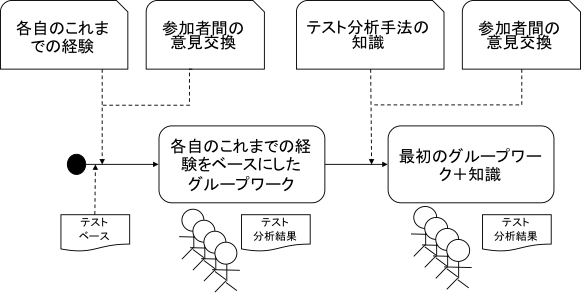
\includegraphics[width=10cm]{./image/D-3-ExparimentAbst1.png}
\caption{演習の前提条件の変化}
\label{fig:D-3-ExparimentAbst1}
\end{center}
\end{figure}

\subsection{実験の題材}
実験の題材は2種類用意した.
[グループ単位1]では,組込みソフトウェア開発の演習題材として音楽再生機器を使った.
フィーチャセットはボリュームコントロールである.2.4.5節で行なった実験とは別の製品の仕様書を題材にしている.
[グループ単位2]では,エンタープライズシステム開発の演習題材として,フライト予約Webシステムを利用した.
フィーチャセットは新規フライト予約である.
テストベースとなる仕様書として,両方とも12枚のパワーポイントのスライドを用意した.
講師側が用意した解答例である,テスト分析で特定すべきテスト条件の一覧を表~\ref{tab:D-3-ensyu1}と表~\ref{tab:D-3-ensyu2}に示す.

% Table generated by Excel2LaTeX from sheet 'Sheet1'
\begin{table}[htbp]
 \footnotesize
  \centering
  \caption{音楽再生機器の講師解答例}
% Table generated by Excel2LaTeX from sheet 'Sheet1'
    \begin{tabular}{|c|l|p{11em}|p{11em}|}
    \hline
    \multicolumn{1}{|p{7em}|}{{論理的機能構造}} & \multicolumn{1}{p{8em}|}{{テストカテゴリ}} & {仕様項目} & {期待結果/確認内容} \bigstrut\\
    \hline
    \hline
    \multicolumn{1}{|c|}{\multirow{2}[4]{*}{{入力調整}}} & \multicolumn{1}{p{7.75em}|}{{対向機入力}} & {--} & {--} \bigstrut\\
\cline{2-4}          & \multicolumn{1}{p{7.75em}|}{{ボタン}} & {・キューイング} & {・早押ししたとき無視すること} \bigstrut\\
    \hline
    \multicolumn{1}{|c|}{\multirow{2}[4]{*}{{出力調整}}} & \multicolumn{1}{p{7.75em}|}{{音声出力}} & {・ボリューム上限下限を知らせるビープ音} & {・ビープ音が押下に対して1回なること} \bigstrut\\
\cline{2-4}          & \multicolumn{1}{p{7.75em}|}{{LED点灯}} & {--} & {--} \bigstrut\\
    \hline
    \multicolumn{1}{|c|}{\multirow{2}[4]{*}{{変換}}} & \multicolumn{1}{p{7.75em}|}{{音量}} & {・音量調節} & {・ボタン押下でボリュームが上下すること} \bigstrut\\
\cline{2-4}          & \multicolumn{1}{p{7.75em}|}{{対向機操作}} & {--} & {--} \bigstrut\\
    \hline
    \multicolumn{1}{|c|}{\multirow{2}[2]{*}{{貯蔵}}} & \multicolumn{1}{l|}{\multirow{2}[2]{*}{{設定保存}}} & {・デフォルト値} & {・ボリュームを変更させてリセットするとデフォルト値に戻ることで確認} \bigstrut[t]\\
          &       & {・音量調節の保存} & {・PowerON後前回Offした際の結果と同じ音量がでることを確認する} \bigstrut[b]\\
    \hline
    \multicolumn{1}{|p{5.835em}|}{{サポート}} & \multicolumn{1}{p{7.75em}|}{{ヘッドセット状態遷移}} & {・状態により音量調節アクションを受け付ける/受け付けない} & {・再生中,通話中以外音量調節ボタンを無視する} \bigstrut\\
    \hline
    \multicolumn{1}{|c|}{\multirow{3}[4]{*}{{相互作用}}} & \multicolumn{1}{p{7.75em}|}{{対向機への反映}} & {・対向機のボリューム値への影響} & {・ヘッドセットのボリュームを変更したあと,対向機のボリュームが変更していないことで確認} \bigstrut\\
\cline{2-4}          & \multicolumn{1}{l|}{\multirow{2}[2]{*}{{設定情報の共有}}} & {・複数の設定情報の設定影響} & {・通話と再生で交互に音量を調節した際に互いに影響を受けないこと} \bigstrut[t]\\
          &       & {・他の処理で音量設定の削除} & {・初期化,リセットで初期値に戻ることを確認} \bigstrut[b]\\
    \hline
    \end{tabular}%
  \label{tab:D-3-ensyu1}%
\end{table}%



% Table generated by Excel2LaTeX from sheet 'Sheet1'
\begin{table}[htbp]
\footnotesize
  \centering
  \caption{フライト予約システムの講師解答例}
    \begin{tabular}{|c|l|p{10.5em}|p{13em}|}
    \hline
    \multicolumn{1}{|p{7em}|}{論理的機能構造} & \multicolumn{1}{p{7em}|}{テストカテゴリ} & 仕様項目  & 期待結果/確認内容 \bigstrut\\
    \hline
    \hline
    \multicolumn{1}{|c|}{\multirow{9}[4]{*}{入力調整}} & \multicolumn{1}{l|}{\multirow{8}[2]{*}{画面入力}} & ・画面表示内容 & ・画面仕様書に沿ったレイアウトであること \bigstrut[t]\\
          &       & ・年,月,日の入力範囲チェック & ・入力フィールド/ボタンの制御が仕様どおりであること \\
          &       & ・入力桁数チェック & ・Min日以降Max日が入力できること\\
          &       & ・型チェック & ・フライト予約可能日以前の入力はクリアされること\\
          &       & ・うるう年判定,末日判定 & ・桁数/文字数チェックをすること\\
          &       & ・出発地と到着地の組み合わせ & ・型(文字,数値)のチェックをすること\\
          &       & \multicolumn{1}{r|}{} & ・うるう年,末日判定のチェックをすること \\
          &       & \multicolumn{1}{r|}{} & ・同じ出発地と到着地を選択できないこと \bigstrut[b]\\
\cline{2-4}          & \multicolumn{1}{p{7.75em}|}{ボタン操作} & ・画面遷移 & ・画面仕様書に沿った画面の遷移ができること \bigstrut\\
    \hline
    \multicolumn{1}{|c|}{\multirow{6}[4]{*}{出力調整}} & \multicolumn{1}{l|}{\multirow{5}[2]{*}{結果表示}} & ・プログレスバー/登録完了メッセージ & ・登録中と登録後表示が正しいこと \bigstrut[t]\\
          &       & ・注文不成立メッセージ & ・メッセージが出ること \\
          &       & ・金額計算表示 & ・フィールドに収まること \\
          &       & ・注文番号 & ・同上 \\
          &       & ・フライト情報 & ・同上\bigstrut[b]\\
\cline{2-4}          & \multicolumn{1}{p{7.75em}|}{帳票出力} & --    & -- \bigstrut\\
    \hline
    \multicolumn{1}{|c|}{\multirow{3}[2]{*}{変換}} & \multicolumn{1}{l|}{\multirow{4}[2]{*}{計算}} & ・合計額の計算 & ・クラス単価×人数となること \bigstrut[t]\\
          &       & ・登録時の採番 & ・直前のNo+1となること \\
          &       & ・チケット在庫の計算 & ・在庫数から購入数をマイナスし0以下にできない \\
    \hline
    \multicolumn{1}{|c|}{\multirow{2}[4]{*}{貯蔵}} & \multicolumn{1}{p{7.75em}|}{検索} & ・フライト検索結果 & ・検索条件(and)で該当するフライトが検索されること \bigstrut\\
\cline{2-4}          & \multicolumn{1}{p{7.75em}|}{登録,更新,削除} & ・フライトの登録 & ・フライトが登録が出来ること \bigstrut\\
    \hline
    \multicolumn{1}{|c|}{\multirow{2}[2]{*}{サポート}} & \multicolumn{1}{l|}{\multirow{2}[2]{*}{エラー処理}} & ・登録時にチケット在庫なし & ・エラーになること\bigstrut[t]\\
          &       & ・注文挿入中の強制終了 & ・ロールバックすること \bigstrut[b]\\
    \hline
    \multicolumn{1}{|c|}{\multirow{3}[2]{*}{相互作用}} & \multicolumn{1}{l|}{\multirow{3}[2]{*}{反映}} & ・「既存注文開く」への反映 & ・検索条件(and)で検索されること \bigstrut[t]\\
          &       & ・「注文件数グラフ」への反映 & ・注文件数がプラスされること \\
          &       & ・「注文履歴」への反映 & ・全ての状況(登録)が書き込まれること \bigstrut[b]\\
    \hline
    \end{tabular}%
  \label{tab:D-3-ensyu2}%
\end{table}%

\subsection{テストカテゴリベースドテスト適用前のテスト分析の結果}

テストカテゴリベースドテストの知識を与えていないため,ルールがない状態で行われたテスト分析結果のばらつきについて,実験による典型的な4パターンのテスト分析結果を図 ~\ref{fig:D-3-Fig1-1}から図 ~\ref{fig:D-3-Fig1-4}で示す.
\begin{enumerate}
\item CS1 と CS2:両方ともテスト対象の入力フィールドを行タイトルに列挙している.しかしながら列名と表の内容が異なっている.
\item CS3: 表の中に記載されている各列,アクションとパラメータと期待結果などが独立しているため,それぞれの間の関連を特定できない.
\item CS4: テスト対象の状態が列名として列挙されている.各状態で取りうるパラメータと値が表の中に記載されている.
\end{enumerate}

この結果は複数の個人のテスト分析が,それぞれ複数の結果に到達することを示している.
複数の結果とは,テスト分析を通して特定したテスト条件にばらつきがあることを意味している.
テスト分析が多くの人たちで行われるときには,テスト条件の重複,もしくは完全に抜け落ちるといった可能性が考えられる.


\begin{figure}[H]
\centering
\subfloat[テスト分析の事例:CS1]{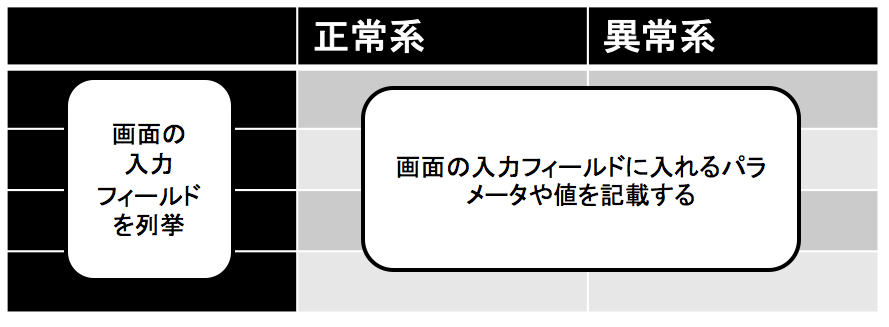
\includegraphics[clip, width=4in]{./image/D-3-Fig1-1.png}
\label{fig:D-3-Fig1-1}}
\\
\subfloat[テスト分析の事例:CS2]{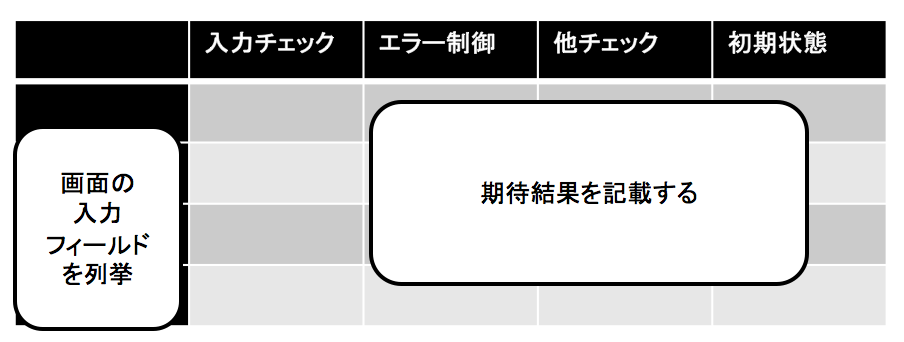
\includegraphics[clip, width=4in]{./image/D-3-Fig1-2.png}
\label{fig:D-3-Fig1-2}}
\\
\subfloat[テスト分析の事例:CS3]{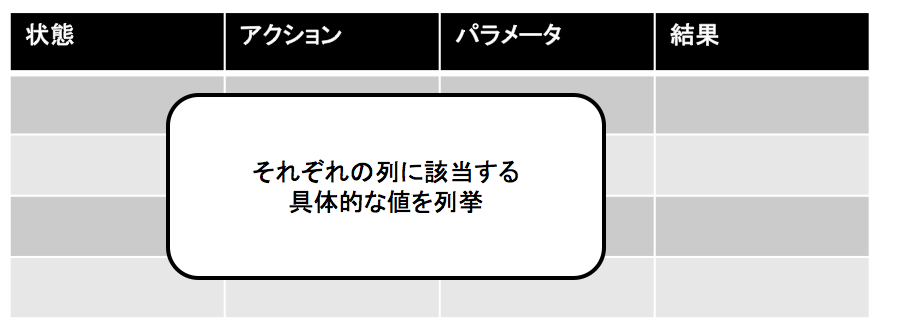
\includegraphics[clip, width=4in]{./image/D-3-Fig1-3.png}
\label{fig:D-3-Fig1-3}}
\\
\subfloat[テスト分析の事例:CS4]{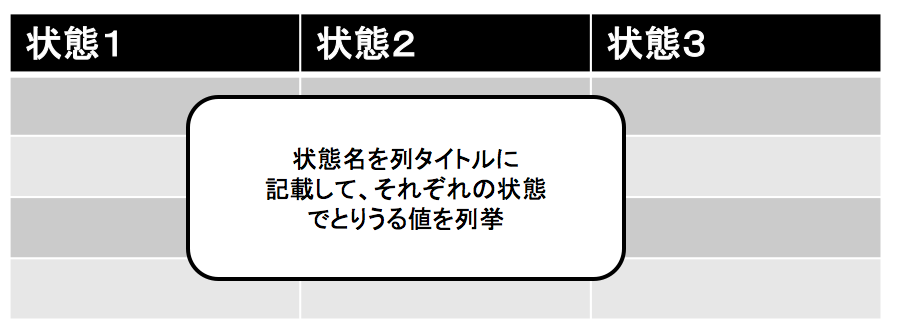
\includegraphics[clip, width=4in]{./image/D-3-Fig1-4.png}
\label{fig:D-3-Fig1-4}}
\caption{ルールがない状態でのテスト分析の事例}
\label{fig:D-3-Fig1-1234}
\end{figure}


\subsection{実験結果の評価}
1回目,2回目の実験では,グループでの解答を実験結果として利用した.
1回目の実験は,組み込み開発を行なっている組織内での6グループの実験結果を収集し,
2回目の実験結果ではオープンセミナーの参加者をグルーピングした2つの実験結果を収集したので,合計で8つの実験結果を収集した.
%題材は,1回目の実験では音楽再生機器をテスト対象の$AS$にした.
%2回目の実験では,飛行機予約システムをテスト対象の$AS$にした.
テストカテゴリベースドテストの知識をを与える前の演習結果と,知識を与えた後の演習結果とを比較した.
テストカテゴリベースドテストの知識を与える前にテスト分析をした結果は,図~\ref{fig:D-3-Fig1-1234}のようにばらつくので,ワークショップの後に講師が仕様項目の数を計算できるように仕様項目の分類をしている.

% Table generated by Excel2LaTeX from sheet '途中経過'
\begin{table}[htbp]
  \centering
  \caption{1回目の実験のグループ2(TM2)での比較結果 }
    \begin{tabular}{|l|r|r|r|r|}
    \hline
    \multirow{2}[4]{*}{テストカテゴリ} & \multicolumn{2}{c|}{期待結果数} & \multicolumn{2}{c|}{パラメータ数} \bigstrut\\
\cline{2-5}          & \multicolumn{1}{l|}{適用なし} & \multicolumn{1}{l|}{適用あり} & \multicolumn{1}{l|}{適用なし} & \multicolumn{1}{l|}{適用あり} \bigstrut\\
    \hline
    \hline
    入力A   & \multicolumn{1}{l|}{N/A} & \multicolumn{1}{l|}{N/A} & \multicolumn{1}{l|}{N/A} & \multicolumn{1}{l|}{N/A} \bigstrut\\
    \hline
    \multirow{2}[4]{*}{変換A} & 1     & 1     & 3     & 3 \bigstrut\\
\cline{2-5}          & 0     & 1     & 0     & 3 \bigstrut\\
    \hline
    変換B   & 0     & 0     & 0     & 0 \bigstrut\\
    \hline
    サポートA & 0     & 0     & 6     & 0 \bigstrut\\
    \hline
    \multirow{2}[4]{*}{サポートB} & 0     & 0     & 0     & 0 \bigstrut\\
\cline{2-5}          & 0     & 0     & 0     & 0 \bigstrut\\
    \hline
    出力A   & 1     & 1     & 2     & 2 \bigstrut\\
    \hline
    出力B   & 0     & 0     & 0     & 0 \bigstrut\\
    \hline
    貯蔵A   & 0     & 1     & 0     & 1 \bigstrut\\
    \hline
    貯蔵B   & \multicolumn{1}{l|}{N/A} & \multicolumn{1}{l|}{N/A} & \multicolumn{1}{l|}{N/A} & \multicolumn{1}{l|}{N/A} \bigstrut\\
    \hline
    \multirow{2}[4]{*}{相互作用A} & 0     & 1     & 0     & 2 \bigstrut\\
\cline{2-5}          & \multicolumn{1}{l|}{N/A} & \multicolumn{1}{l|}{N/A} & \multicolumn{1}{l|}{N/A} & \multicolumn{1}{l|}{N/A} \bigstrut\\
    \hline
    合計    & 2     & 5     & 11    & 11 \bigstrut\\
    \hline
    \end{tabular}%
  \label{tab:D-3-tab3}%
\end{table}%

表~\ref{tab:D-3-tab3}は最初の演習結果のうちの1つグループの結果を比較した表である.
知識を与える前と後では,特定した期待結果の数は2つ増えている.
テストパラメータを特定した数は合計としては変わらないが期待結果と紐つけて特定しているようになっている.
サポートにかかるテストパラメータに関してだけ,知識を与える前よりも減っている.
このテスト条件は,状態により処理を受け付ける場合と受け付けなくなる場合があることを確認するテスト条件である.
知識を与える前は,状態を6つ列挙していたが,期待結果の記載がなかった.
知識を与えた後は,列挙していた状態に関する記述がなくなっていた.
グループの人員に確認したところ,期待結果が不明であるために記載するのを辞めたことが理由であった.

% Table generated by Excel2LaTeX from sheet 'Sheet1'
\begin{table}[htbp]
%\footnotesize
  \centering
  \caption{評価レベルの定義}
    \begin{tabular}{|l|p{14em}|}
       \hline
    評価レベル & \multicolumn{1}{l|}{比較結果} \\
        \hline
        \hline
     B    & リストしたテスト条件数は増加していない, かつ実験の期待結果よりも少ない.  \\
        \hline
    -     & リストしたテスト条件数は増加していない, しかしすでに期待結果と同数である.  \\
        \hline
    A     & リストしたテスト条件数は増加している, しかし実験の期待結果よりも少ない.   \\
       \hline
    A${}^\text{+}$    & リストしたテスト条件数は増加している, かつ実験の期待結果に達している. \\
        \hline
    \end{tabular}%
  \label{tab:D-3-tab4}%
\end{table}%

8つの実験結果を比較するために,表~\ref{tab:D-3-tab4}に示した評価レベルを設定した.
評価レベルは4段階であり,特定したテスト条件が増加し,期待結果に達しているA${}^\text{+}$ が最も高い.
最も低いレベルはBで,特定したテスト条件が増加せず,かつ期待結果よりも少ない場合である.

検証実験にて収集した8つのグループの評価結果を表~\ref{tab:D-3-tab5}に示す.
TM1からTM6までが最初の実験の結果である.
$AS$は音楽生成機器であり,フィーチャセットはボリュームコントロールである.
この実験結果では,演習の解答例と同じだけのテスト条件を特定できたグループは0であった.
ただし,6グループ中5グループにおいて,列挙したテスト条件の数が増えている.
論理的機能構造の要素ごとの比較では,相互作用にて5グループの列挙数が増加している.
出力調整と貯蔵では,列挙数が増加したグループ以外は特定すべき仕様項目がすでに最初の演習で列挙できているため,効果があったかどうかはこの結果からは判断できない.
ただし,サポートは全グループにてテスト条件の増加がないため,効果は出ていないと考えられる.

\begin{table}[htbp]
\footnotesize
  \centering
  \caption{検証実験のグループごとの評価結果}
    \begin{tabular}{|l|l|l|l|l|l|l|l|l|}
    \hline
    \multicolumn{1}{|c|}{\multirow{2}[4]{*}{論理的機能構造}} & \multicolumn{8}{c|}{グループ} \bigstrut\\
\cline{2-9}          & TM1   & TM2   & TM3   & TM4   & TM5   & TM6 & TM7 & TM8 \bigstrut\\
    \hline
    \hline
    変換  & B     & A     & B     & B     & B     & B & A     & A\bigstrut\\
    \hline
    入力 &  -     &   -     &   -    &   -    &   -    & -     & A     & B   \bigstrut\\
    \hline
    出力 & -     & -     & -     & -     & -     & A${}^\text{+}$ & A     & A \bigstrut\\
    \hline
    貯蔵 & -     & A${}^\text{+}$    & -     & A${}^\text{+}$    & A${}^\text{+}$    & -& A     & A  \bigstrut\\
    \hline
    サポート & B     & B     & B     & B     & B     & B& B     & A \bigstrut[t]\\
    \hline
    相互作用  & B     & A     & A     & A${}^\text{+}$    & A     & A${}^\text{+}$& B     & A \bigstrut[b]\\
    \hline
    \end{tabular}%
  \label{tab:D-3-tab5}%
\end{table}%

TM7とTM8は2回目の実験である.
$AS$はフライト予約システムである.
新規フライト予約がフィーチャセットである.
この実験でも知識を与えた後の演習結果にて解答例と同じ数のテスト条件を特定したグループはいなかった.
ただし,2グループ全てにおいてテストカテゴリ内に列挙したテスト条件の数が増えている.
論理的機能構造の要素ごとの比較では,変換と出力調整と貯蔵にて2グループともにテスト条件の列挙数が増えた.
それ以外の要素では1グループのみが列挙数が増えた結果となっている.

全体的に定量的な向上が見られたが,特定のグループの著しい成長,もしくは論理的機能構造の要素毎に特徴的な傾向は見出せなかった.
サンプルとなるデータ数が8つと少ないため,3回目の検証実験では,実験データ取得の方法を変更した.

\newpage
\section{個人単位の実験}
\subsection{実験の概要}
3回目の検証実験では,グループ単位ではなく,各参加者の実施結果を収集した\cite{yumoto2016ICST}.
\begin{figure}[h]
\begin{center}
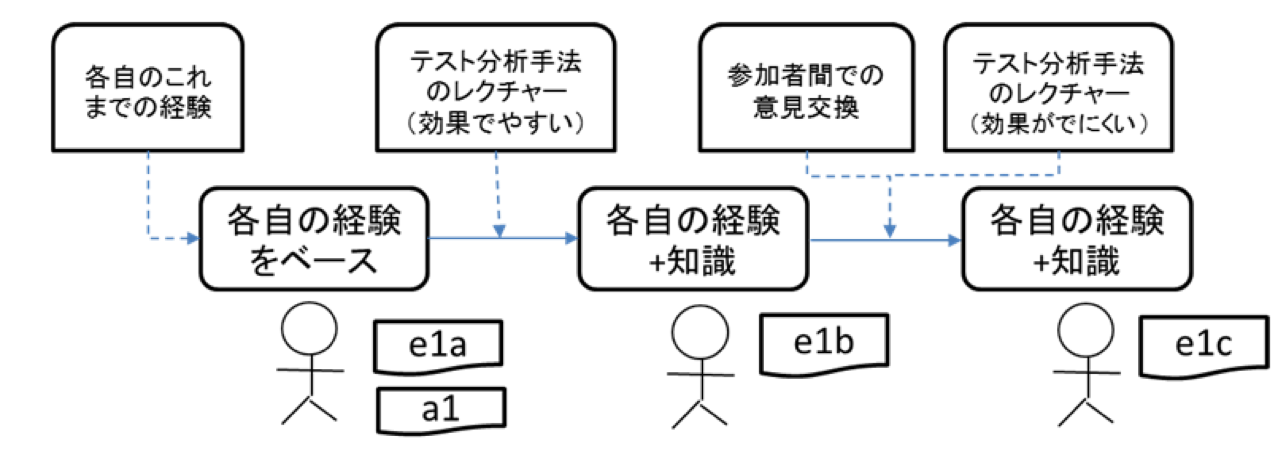
\includegraphics[width=10cm]{./image/D-3-Fig8.png}
\caption{e1aからe1cまでの演習の前提条件の変化}
\label{fig:D-3-Fig8}
\end{center}
\end{figure}
ワークショップを通して,図~\ref{fig:D-3-Fig8}のように,知識を与えていない状態での演習実施(e1a),
一部分だけ知識を与えた状態で演習実施(e1b),
全てを知識を与えた状態で演習実施を(e1c)行い,各参加者の演習結果を実験データとして収集した.
e1aのタイミングで記述式のアンケート(a1)をとっている.

テストカテゴリベースドテストのレクチャーを2回に分けた理由は, 前述したように手法の実施手順がデータフローを使った手順とそれ以外の手順に分けられるため, 2段階にわけることがワークショップの参加者にとって知識習得が容易になるであろうという判断からである.

\begin{figure}[h]
\begin{center}
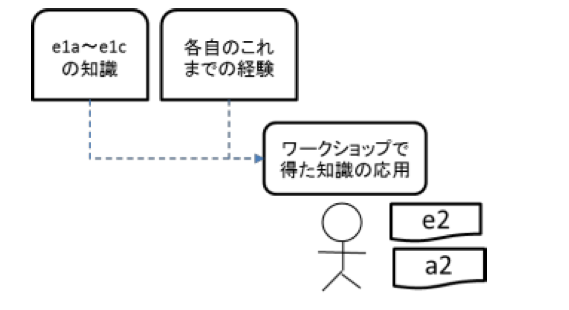
\includegraphics[width=9cm]{./image/D-3-Fig9.png}
\caption{e2 の演習の前提条件の変化}
\label{fig:D-3-Fig9}
\end{center}
\end{figure}
e2 では,図~\ref{fig:D-3-Fig9}のように,e1a からe3a までで行ったレクチャーと演習を通じて得た知識とスキルが別の題材で活用できることを確認する. e1a と比較することで, スキルが向上しているかを観察する.
1cの後には再度アンケート(a2)をとっている.

このワークショップでは,57名分のIT技術者が参加した.
参加者の年齢,業務領域,経験年数とテスト技法の知識は図~\ref{fig:D-3-Fig6},図~\ref{fig:D-3-Fig7},図~\ref{fig:D-3-Fig7b}のとおりである.
年齢構成,業務領域ともに偏りがなく,産業界のサンプリングとして意味があると考える.

\begin{figure}[H]
\begin{center}
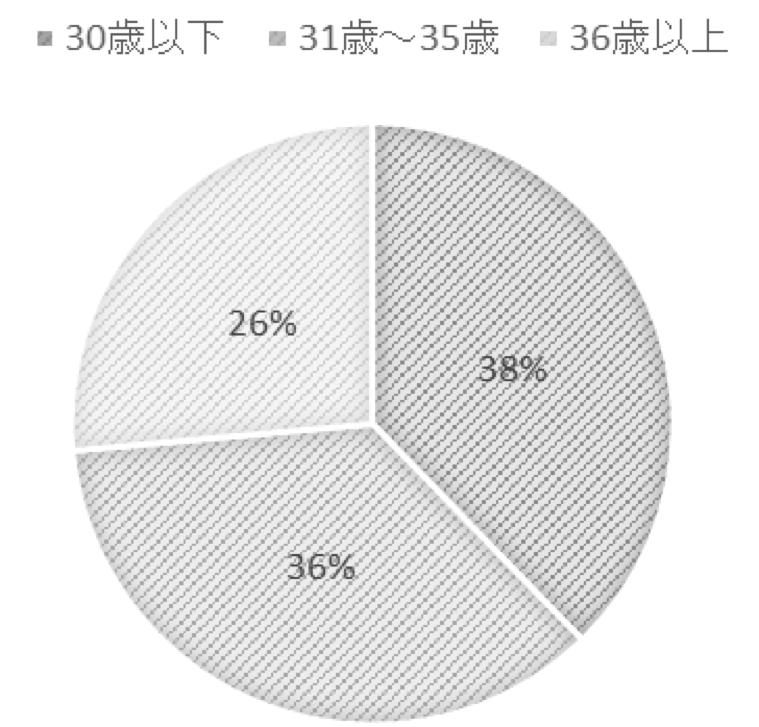
\includegraphics[width=8cm]{./image/D-3-Fig6.png}
\caption{参加者の年齢分布}
\label{fig:D-3-Fig6}
\end{center}
\end{figure}

\begin{figure}[H]
\begin{center}
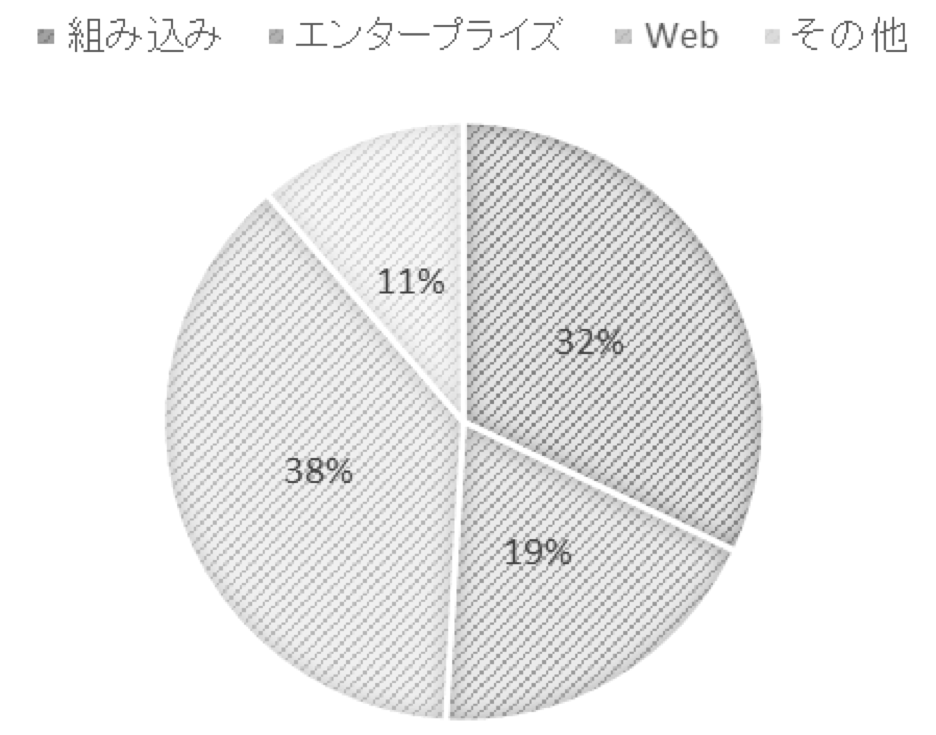
\includegraphics[width=10cm]{./image/D-3-Fig7.png}
\caption{参加者の業務領域分布}
\label{fig:D-3-Fig7}
\end{center}
\end{figure}

参加者の技術経験と,テスト技法の研修受講有無(テスト技法に関する知識習得)については,a1にて記述式のアンケートにて確認を行った.
テスト技法の研修受講経験のある技術者が38人と半分以上をしめているのが,いままでの実験の被験者とは異なる.
このワークショップ参加者の特徴として,今までに何らかの研修を受けた経験が一般的な技術者と比較して多いことがあげられる.
この理由は,このワークショップは実費を参加者自身が支払い,土日を費やして実施するものであるためで,参加者のキャリア意識が高いことにある.

\begin{figure}[H]
\begin{center}
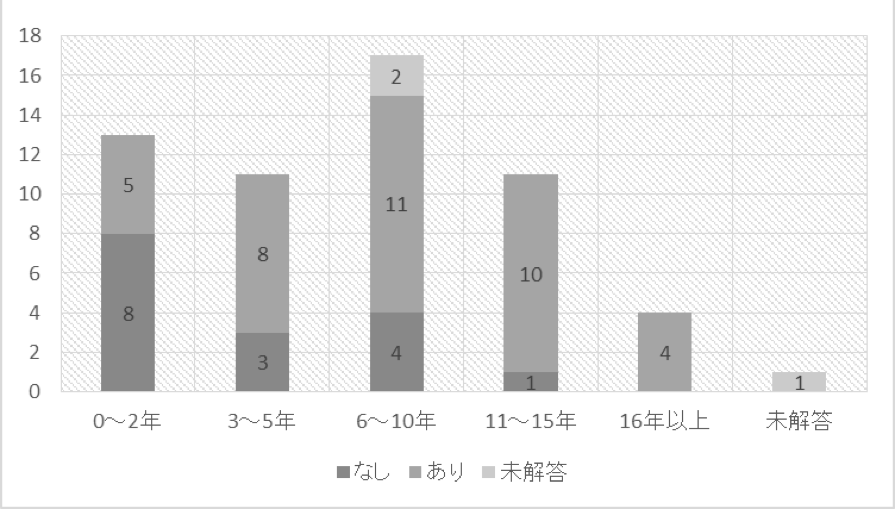
\includegraphics[width=10cm]{./image/D-3-Fig7b.png}
\caption{実務経験とテスト技法研修受講実績}
\label{fig:D-3-Fig7b}
\end{center}
\end{figure}



\subsection{実験の題材}
演習題材は,組み込みソフトウェア開発とエンタープライズシステム開発のシステムレベルの仕様を用意した.
組み込みソフトウェア開発の演習題材は音楽再生用機器のボリュームコントロールをフィーチャセットとしたものである.
3.2節の[グループ単位1]の演習で利用した題材と同じものである.
エンタープライズシステム開発の演習題材は,フライト予約システムの新規フライト予約をフィーチャセットとして演習問題を用意した.
3.2節の[グループ単位2]の演習で利用した題材と同じものである.
講師側が用意した解答例である,テスト分析で特定すべきテスト条件の一覧は,3.2節同様に表~\ref{tab:D-3-ensyu1}と表~\ref{tab:D-3-ensyu2}となる.


\subsection{実験結果の評価} \label{sec:3-2}
e1a,e1b,e1c,e2 の演習結果において,各参加者が特定できたテスト条件数 (解答数) を図~\ref{fig:D-3-Fig10}の箱ひげ図を用いて比較する.
図~\ref{fig:D-3-Fig10}のY軸は解答したテスト条件数を示し,X 軸は,各演習における解答数の分布を箱ひげ図で示している.

%箱ひげ図 %<図7 参加者あたりのテスト条件特定数>
\begin{figure}[htbp]
  \begin{center}
  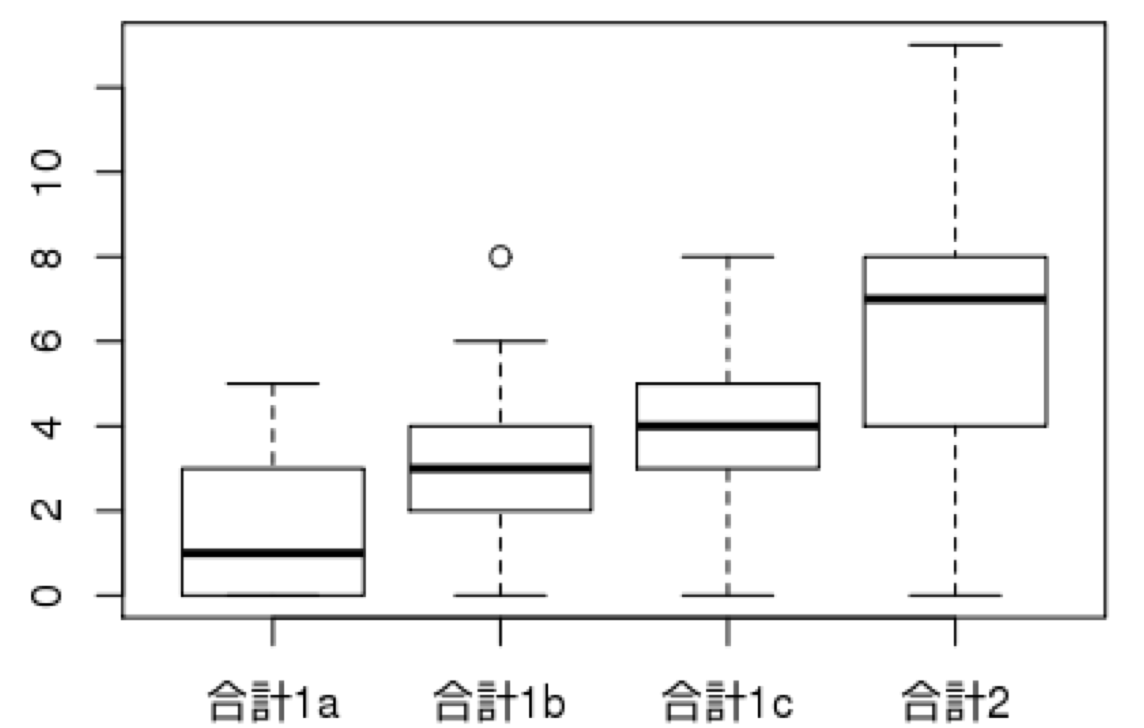
\includegraphics[width=10cm]{./image/D-3-Fig10.png}
  \caption{参加者あたりのテスト条件特定数}
  \label{fig:D-3-Fig10}
  \end{center}
\end{figure}

e1aでは,最高点は5であり,中央値は1 であった.
正解数とした数は9なので,非常に低い値であった.
レクチャー後のe1bでは中央値が3,e1c では4,e2 では7 と,演習が進むごとに中央値が増えているので,テスト条件数を特定するスキルが向上したと考えられる.
ただし,e2 とそれ以外は演習題材が異なり,正解とした条件数が異なる(e1は9で,e2 は24 である).
そのため,単純な数値の比較では不十分である.
正解とするケース数を100 とした箱ひげ図を図~\ref{fig:D-3-Fig11}に示す.
%<図8 参加者あたりのテスト条件特定割合>
\begin{figure}[htbp]
  \begin{center}
  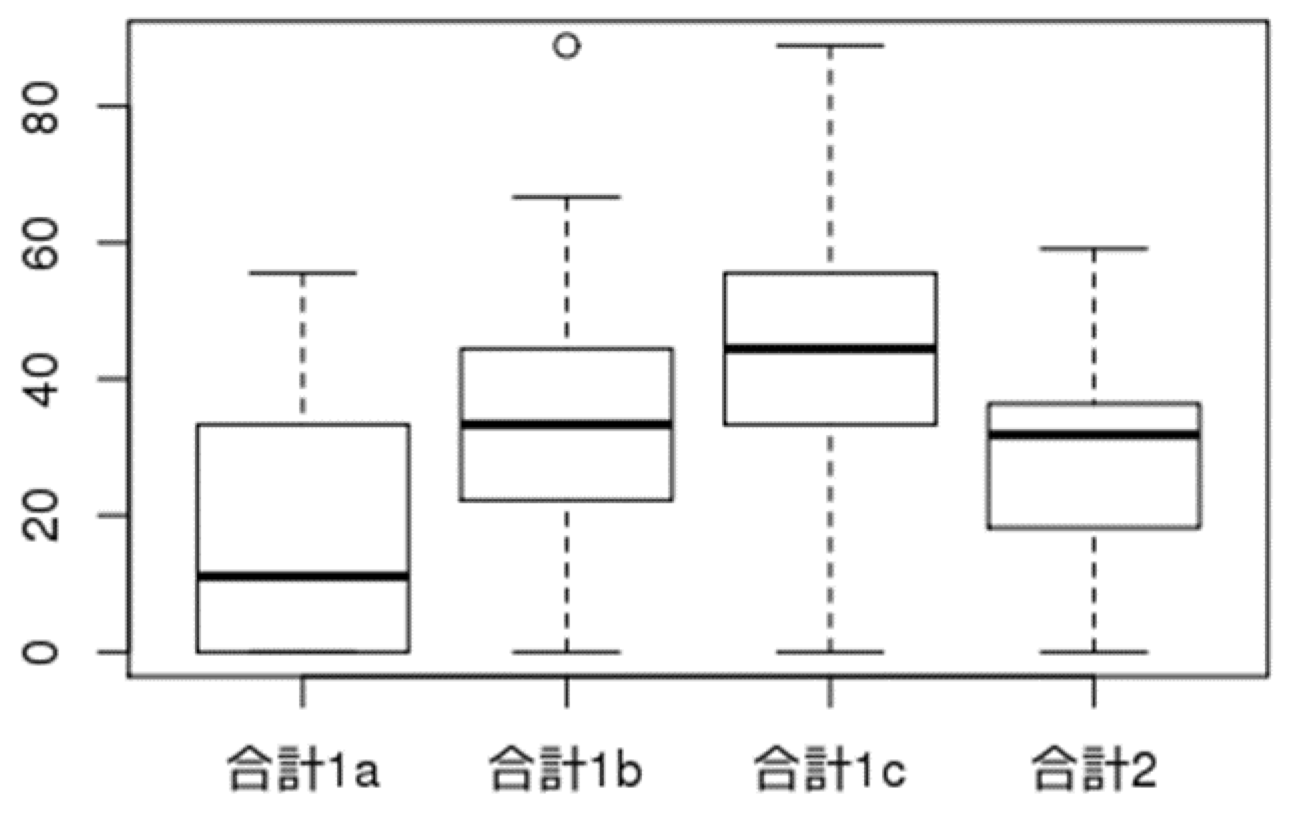
\includegraphics[width=10cm]{./image/D-3-Fig11.png}
  \caption{参加者あたりのテスト条件特定割合}
  \label{fig:D-3-Fig11}
  \end{center}
   \end{figure}

図~\ref{fig:D-3-Fig11}からは, e1a では約10パーセントであったテスト条件の特定数の割合の中央値が,e2 では約40パーセントまで向上したことが確認できる.
ただし,図~\ref{fig:D-3-Fig10}と図~\ref{fig:D-3-Fig11}からわかるように参加者全員のテスト条件特定数が一律に上がったわけではない.
効果があった部分とそうでない部分がどこであるかを調べるために,テスト条件ごとの特徴,および参加者の特徴でさらに分析をすすめた.

\begin{figure}[htbp]
  \begin{center}
  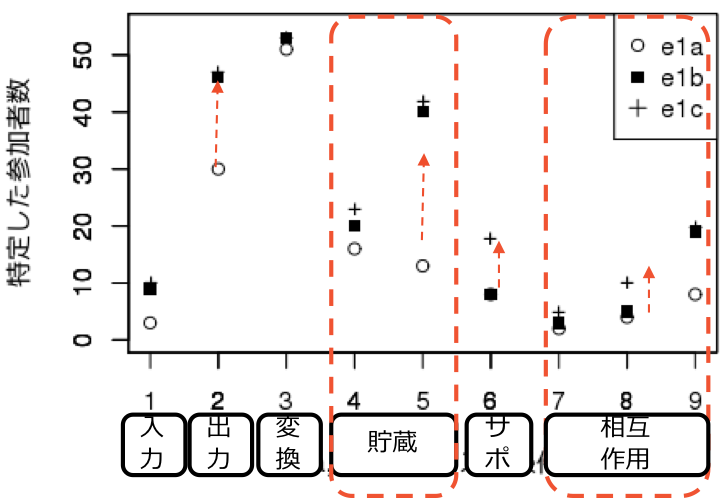
\includegraphics[width=10cm]{./image/D-3-Fig12-1.png}
  \caption{e1aからe1cまでの演習解答の分布}
  \label{fig:D-3-Fig12-1}
  \end{center}
\end{figure}
各参加者が特定できたテスト条件数 (解答数) を図\ref{fig:D-3-Fig12-1}のように論理的機能構造で分類して比較した.
図\ref{fig:D-3-Fig12-1}のY軸はテスト条件毎に解答できた参加者数を示し,X軸は,テスト条件を示している.
1a,1b,1c と進むにつれて,分析で特定できるテスト条件が増えていることがわかる.
テストカテゴリベースドテストの知識を与えることで特に伸びたのは,出力と貯蔵に属するテスト条件であった.

\begin{table}[htbp]
%  \footnotesize
  \centering
  \caption{e1a からe1c までの演習結果の変化}
    \begin{tabular}{rrrrr}
    \hline
    \multicolumn{1}{|l|}{} & \multicolumn{1}{p{7em}|}{論理的機能構造} & \multicolumn{1}{p{7em}|}{テストカテゴリ} & \multicolumn{1}{p{4.5em}|}{難しさ} & \multicolumn{1}{p{4.5em}|}{効果} \bigstrut\\
    \hline
    \hline
    \multicolumn{1}{|l|}{1} & \multicolumn{1}{p{6em}|}{入力調整} & \multicolumn{1}{p{6em}|}{ボタン} & \multicolumn{1}{p{6em}|}{難} & \multicolumn{1}{p{6em}|}{中} \bigstrut\\
    \hline
    \multicolumn{1}{|l|}{2} & \multicolumn{1}{p{6em}|}{出力調整} & \multicolumn{1}{p{6em}|}{音声出力} & \multicolumn{1}{p{6em}|}{中} & \multicolumn{1}{p{6em}|}{高} \bigstrut\\
    \hline
    \multicolumn{1}{|l|}{3} & \multicolumn{1}{p{6em}|}{変換} & \multicolumn{1}{p{6em}|}{音量} & \multicolumn{1}{p{6em}|}{易} & \multicolumn{1}{p{6em}|}{低} \bigstrut\\
    \hline
    \multicolumn{1}{|l|}{4} & \multicolumn{1}{l|}{\multirow{2}[4]{*}{貯蔵}} & \multicolumn{1}{p{6em}|}{設定保存1} & \multicolumn{1}{p{6em}|}{難} & \multicolumn{1}{p{6em}|}{中} \bigstrut\\
\cline{1-1}\cline{3-5}    \multicolumn{1}{|l|}{5} & \multicolumn{1}{l|}{} & \multicolumn{1}{p{6em}|}{設定保存2} & \multicolumn{1}{p{6em}|}{難} & \multicolumn{1}{p{6em}|}{高} \bigstrut\\
    \hline
    \multicolumn{1}{|l|}{6} & \multicolumn{1}{p{6em}|}{サポート} & \multicolumn{1}{p{6em}|}{状態遷移} & \multicolumn{1}{p{6em}|}{難} & \multicolumn{1}{p{6em}|}{中} \bigstrut\\
    \hline
    \multicolumn{1}{|r|}{7} & \multicolumn{1}{l|}{\multirow{3}[6]{*}{相互作用}} & \multicolumn{1}{p{6em}|}{対向機反映} & \multicolumn{1}{p{6em}|}{難} & \multicolumn{1}{p{6em}|}{低} \bigstrut\\
\cline{1-1}\cline{3-5}    \multicolumn{1}{|r|}{8} & \multicolumn{1}{l|}{} & \multicolumn{1}{p{6em}|}{設定共有1} & \multicolumn{1}{p{6em}|}{難} & \multicolumn{1}{p{6em}|}{中} \bigstrut\\
\cline{1-1}\cline{3-5}    \multicolumn{1}{|r|}{9} & \multicolumn{1}{l|}{} & \multicolumn{1}{p{6em}|}{設定共有2} & \multicolumn{1}{p{6em}|}{難} & \multicolumn{1}{p{6em}|}{中} \bigstrut\\
    \hline
    \multicolumn{5}{p{30em}}{難しさ 0-10難 11-25中 26-易} \bigstrut[t]\\
    \multicolumn{5}{p{30em}}{0-10低 11-25中 26-高} \bigstrut[t] \\
    \end{tabular}%
  \label{tab:D-3-tab10}%
\end{table}%

表~\ref{tab:D-3-tab10}は,1から9までのテスト条件を対応する論理的機能構造とテストカテゴリを示し,難しさと知識を与えることによる教育効果を示した.
難しさは,正解数の分布から3段階に分けた.教育効果は,e1a(教育前)とe1c(教育後)の差を3段階で分類した.
表~\ref{tab:D-3-tab10}から,テスト条件2の音声出力と,テスト条件5の設定保存は,演習が進むにつれテスト条件が特定できた参加者が増加したため,特に効果が高かったといえる.これは,過去の実験と同様の結果である.2章にて,仕様書には明確に記述がないものは,テストカテゴリのようなガイドを使うことで特定が容易になるのと仮説をたてて実験を行ったが,今回の実験でもその仮説を実証する結果となった.

続いて,ワークショップ参加者の業務経験年数ごとに,テスト条件を特定できた数にどのような傾向があるかを調査した.ワークショップ参加者の実業務の経験年数はa1でのアンケート結果を利用した.図~\ref{fig:D-3-Fig15}のように,e1aでは,業務経験1~2年の参加者以外は,全ての経験年数で中央値がほぼ同じになった.テスト分析に関して,入社3年でほぼ同様の能力になり,その後は業務経験を重ねてもテストケースを作る能力はあまり変化していない.
入社1~2年では,テスト設計技術に関するスキルの伝達がなされていない,もしくは行われていても効果が出ていないことが推定できる.
%箱ひげ図 %<図7 参加者あたりのテスト条件特定数>
\begin{figure}[htbp]
  \begin{center}
  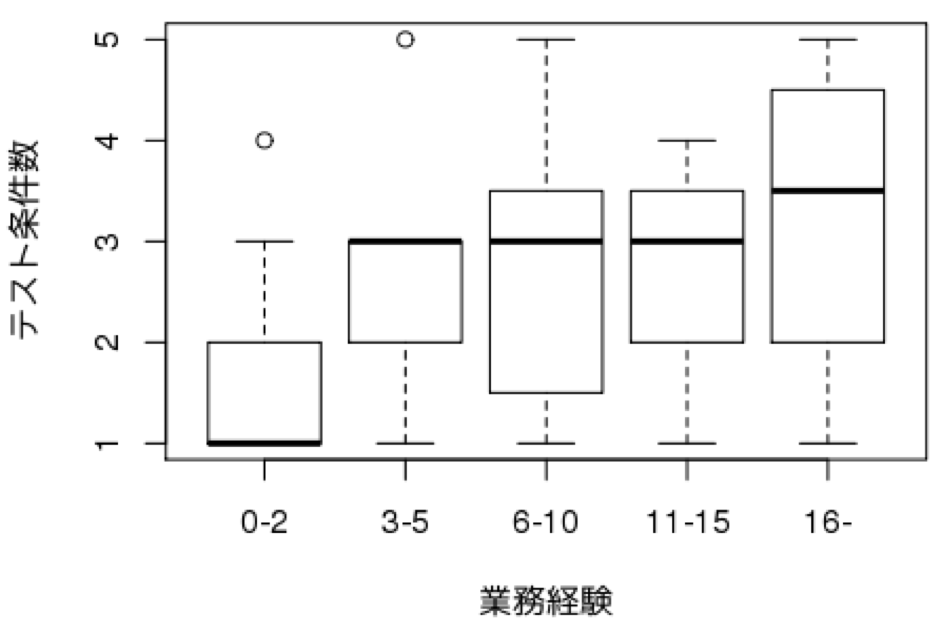
\includegraphics[width=10cm]{./image/D-3-Fig15.png}
  \caption{e1aの参加者/業務経験別テスト条件特定数}
  \label{fig:D-3-Fig15}
  \end{center}
\end{figure}

レクチャーと演習を通じて得たスキルを確認するため,e2aの結果を比較したものが図~\ref{fig:D-3-Fig16}である.全体的に向上しているが,特に業務経験が0-2年度の参加者が伸びたため,業務経験とテスト条件を特定できる能力に差がほとんどなくなってきていることが確認できた.

\begin{figure}[htbp]
  \begin{center}
  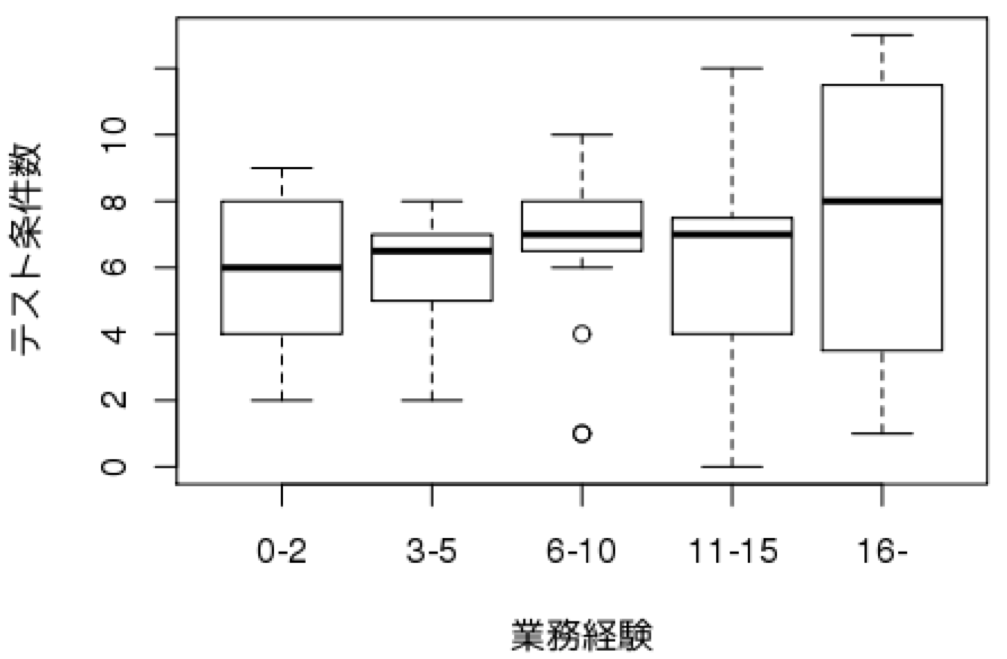
\includegraphics[width=10cm]{./image/D-3-Fig16.png}
  \caption{e2の参加者/業務経験別テスト条件特定数}
  \label{fig:D-3-Fig16}
  \end{center}
   \end{figure}


\subsection{テストカテゴリベースドテスト適用前のテスト分析方法の分類}
今回のワークショップでは, e1aの演習にて,テスト分析結果をこれまでの業務経験に基づいて自由に書いてもらうようにした.
テストカテゴリベースドテストの知識を与える前のときのテスト分析結果から,テスト分析結果の記載は,図\ref{tab:D-3-tab11}に示す通り4つに分類できた.
%<表3 テスト記述パターン>
% Table generated by Excel2LaTeX from sheet 'Sheet4'
\begin{table}[htbp]

  \centering
  \caption{テスト記述パターン}
    \begin{tabular}{|c|p{9em}|p{14em}|p{3em}|}
    \hline
          & パターン & 記載内容 & \multicolumn{1}{c|}{分類} \bigstrut\\
    \hline
    \hline
    1     & 仕様項目  & 「○○な場合に××なること」といったテスト対象の仕様 & 分析的 \bigstrut\\
    \hline
    2     & テストケース & 入力値,アクション,期待結果 & 実装的 \bigstrut\\
    \hline
    3     & P-V(パラメータ/値) & パラメータと値 & 分析的 \bigstrut[t]\\
    \hline
    4     & シナリオ  & 操作手順として記載 & 実装的 \bigstrut[b]\\
    \hline
    \end{tabular}%
  \label{tab:D-3-tab11}%
\end{table}%

表~\ref{tab:D-3-tab11}の1と3は中間成果物的であり,記載した内容を見てそのままテストを実行するには不向きであるが,2と4 はそのままテスト実行時に利用できる.
一方,分析や設計をすると1と3が成果物になる.
自由に記載してもらう際に分析結果から書くことは,普段の業務でも分析や設計をしていると想定できる.
ここから2と4 を直接書くのは,普段の業務であまり分析や設計行為をしていないのではないかという仮説をたてた.
普段から業務にて分析や設計をしている参加者のほうが,分析,設計の活動に慣れているために知識の習得が早いと仮定し,今回のワークショップを通じた演習結果にてこれまでの記載方法と演習の成果に相関があるかを調査した.

\begin{figure}[h]
  \begin{center}
  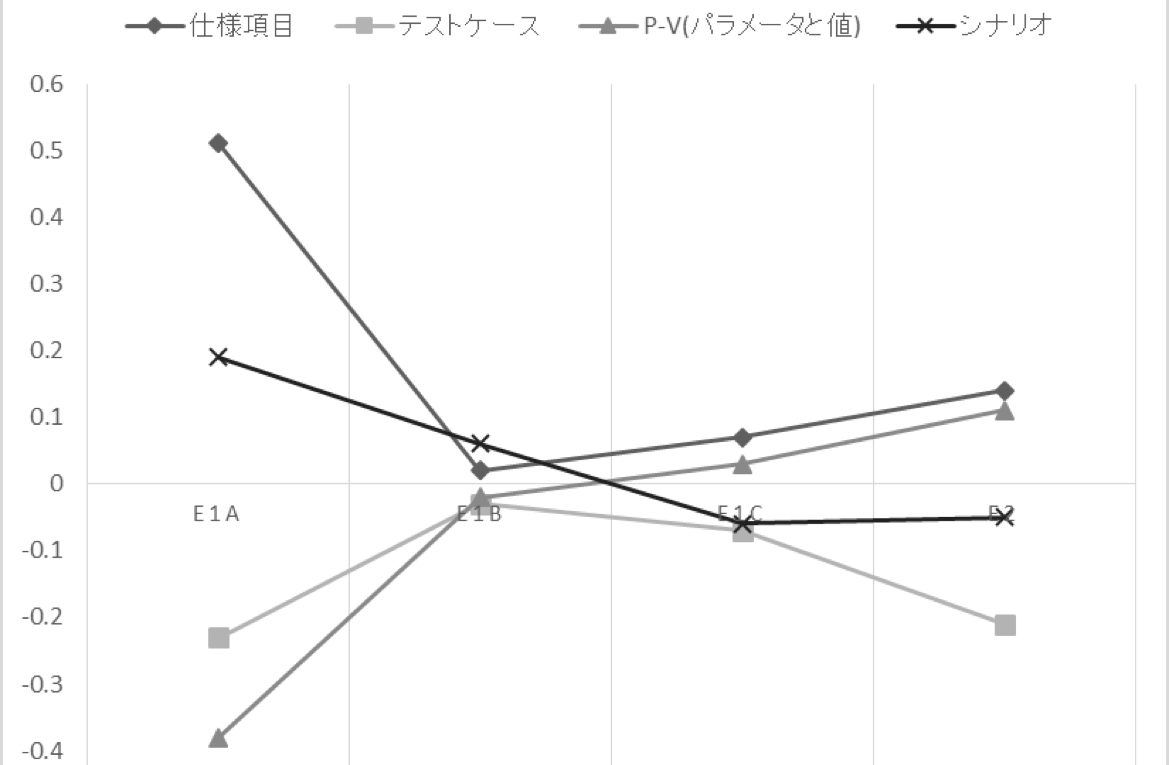
\includegraphics[width=10cm]{./image/D-3-Fig13.png}
  \caption{e1aの参加者業務分野別テスト条件特定数}
  \label{fig:D-3-Fig13}
  \end{center}
\end{figure}

図~\ref{fig:D-3-Fig13} がスピアマンの順序相関分析をした結果である,e1aでは,仕様項目から記載する参加者と特定できたテスト条件数には,0.51(0.4 以上の値は相関ありといえる)の相関が出たたがそれ以外は0.4 以上の値は出なかった.
グラフの傾向からは,e2では分析的な記述をしていた参加者のほうが実装的な記述をした参加者より正の相関となったが,分析結果の値は0.2を割り込んでいるため,相関があるとは結論付けられない.

e1a の仕様項目を記載する参加者だけ相関が出たのは,今回の演習で特定するテスト条件が仕様項目そのものであるため,最初の演習では仕様項目を記載した参加者と結果の相関が出たと考えられる.

\newpage
\section{まとめ}
本章は,3回の予備実験を通して,テストカテゴリベースドテストの知識を与える前のテスト分析での結果のばらつきの傾向,及びばらつきの傾向と分析手法を適用後の結果との相関を調査した.
実験はワークショップを通じてグループ単位で2回,個人単位で1回行なった.
テスト対象を詳細化するときに分類に対する一貫性が欠如していることによるテスト分析結果のばらつきを確認することができた.
また,分類ルールの手法としてテストカテゴリベースドテストの知識を与えることで,テスト条件を特定できる数が増えることが確認できた.仮説として立てた「仕様書には明確に記述がないものは,テストカテゴリのようなガイドを使うことで特定が容易になる」ことが実証できる傾向になった.
ただし,テストカテゴリベースドテストの知識を与えても期待した数のテスト条件を特定できるわけではないことが確認できた.
また,業務経歴3年未満の技術者には有効であったが,3年以上の技術者にはあまり効果が出ないことも確認した.
